\documentclass[11pt]{scrartcl}
\usepackage{fullpage}

\usepackage{listings} % Coding Syntax coloring
\usepackage{color}
\usepackage{textcomp}
\definecolor{listinggray}{gray}{0.9}
\definecolor{lbcolor}{rgb}{0.9,0.9,0.9}

\usepackage{amsmath}
\usepackage{textcomp}

\lstset{
     backgroundcolor=\color{lbcolor},
     tabsize=4,
     rulecolor=,
     language=matlab,
        basicstyle=\scriptsize,
        upquote=true,
        aboveskip={1.5\baselineskip},
        columns=fixed,
        showstringspaces=false,
        extendedchars=true,
        breaklines=true,
        prebreak = \raisebox{0ex}[0ex][0ex]{\ensuremath{\hookleftarrow}},
        frame=single,
        showtabs=false,
        showspaces=false,
        showstringspaces=false,
        identifierstyle=\ttfamily,
        keywordstyle=\color[rgb]{0,0,1},
        commentstyle=\color[rgb]{0.133,0.545,0.133},
        stringstyle=\color[rgb]{0.627,0.126,0.941},
}
\usepackage{fancyhdr,graphicx,lastpage}% http://ctan.org/pkg/{fancyhdr,graphicx,lastpage}
\fancypagestyle{plain}{
  \fancyhf{}% Clear header/footer
  \fancyhead[R]{
\includegraphics[scale=0.5]{logo.png}}% Right header
  \fancyhead[L]{\textbf{School of Electronic and Electrical Engineering}}
  %\fancyfoot[L]{Name Firstname - v1.0 \\  Date}% Left footer
  \fancyfoot[R]{\thepage\  / \pageref{LastPage}}% Right footer
}
\pagestyle{plain}% Set page style to plain.


\begin{document}
\title{ELEC2856 Assignment 2}
\subtitle{ Audio Signal Processing}
\author{Yingjie Luan}
\maketitle

\tableofcontents

\section{C Simulation code}
Below is the simulation code,
\begin{enumerate} 
\item main.c
\begin{lstlisting}[language=C]
#include <stdio.h>

#include "reader.h"
#include "buffer.h"

#define buffer_size 19


void give_weight(double * weight){
    weight[0] = -0.002693840;
    weight[1] = -0.002519748;
    weight[2] =  0.005014695;
    weight[3] =  0.015641050;
    weight[4] =  0.000000000;
    weight[5] = -0.046914239;
    weight[6] = -0.048021820;
    weight[7] =  0.083481298;
    weight[8] =  0.294332820;
    weight[9] =  0.400000000;
    weight[18] = -0.002693840;
    weight[17] = -0.002519748;
    weight[16] =  0.005014695;
    weight[15] =  0.015641050;
    weight[14] =  0.000000000;
    weight[13] = -0.046914239;
    weight[12] = -0.048021820;
    weight[11] =  0.083481298;
    weight[10] =  0.294332820;
}

double cal_elem(double * weight, struct circle * buffer){
    double sum = 0;

    for(int i = 0; i <= buffer_size-1; i++){
        sum += (buffer->num)*weight[i];
        buffer = buffer->next;
    }
    return sum;
}


int main(){
    double weight[buffer_size] = {0};
    give_weight(weight);

    double array[1000] = {0.0};
    array[25] = 1.0;

    struct circle * buffer = create(buffer_size-1,array);
    reader();

    for(int i = buffer_size; i <= 800; i++){
        double current = cal_elem(weight,buffer);
        printf("%lf\n",current);
        buffer = rotate(buffer,array[i]);
    }

}
\end{lstlisting}
\item reader.h:
\begin{lstlisting}[language=C]
#include "stdio.h"

int reader(void);
\end{lstlisting}
\item reader.c
\begin{lstlisting}[language=C]
#include "reader.h"


int reader(void ) {
    FILE * input;
    input = fopen("test", "r");
    if(input == NULL)
    {
        printf("failed\n");
        return -1;
    }

    while(! feof(input)){
        double in_line;
        fscanf( input, "%f\n", in_line );
        printf("%lf",in_line);
    }
    return 0;

}
\end{lstlisting}
\item buffer.h
\begin{lstlisting}[language=C]
#include <stdlib.h>


struct circle{
    float num;
    struct circle * next;
    struct circle * before;
};

struct circle * create(int size,double * array);

struct circle * rotate(struct circle * head, double num);

\end{lstlisting}
\item buffer.c
\begin{lstlisting}[language=C]
#include "buffer.h"

struct circle * create(int size,double * array){
    struct circle * head, *pf, *pb;
    head = (struct circle *) malloc(sizeof(struct circle));
    pb = head;
    for(int i = 0; i<size ; i++){
        pf = (struct circle *) malloc(sizeof(struct circle));
        pb->num = array[i];
        pb->next = pf;
        pf->before = pb;
        pb = pf;
    }
    pb->num = array[size];
    pb->next = head;
    head->before = pb;
    return head;
}

struct circle * rotate(struct circle * head, double num){
    head->num = num;
    return head->next;
}

\end{lstlisting}
\end{enumerate}

\section{Description of the code}
\subsection{What it does at each interrupt?}

At the real implementation time, before the system get into working condition, a buffer is created and initialized. \\

After that, during each interrupt, function \textit{rotate()} and function \textit{cal\_elem()} will be used, and an analog signal will be set according to the return value of function \textit{cal\_elem()}.
\subsection{Implementation of a fixed length queue}

A fixed length queue was implemented to support buffering. The rotation efficiency is O(1).
\begin{center}
\begin{minipage}[t]{\linewidth}
%\label{fig:main}

{
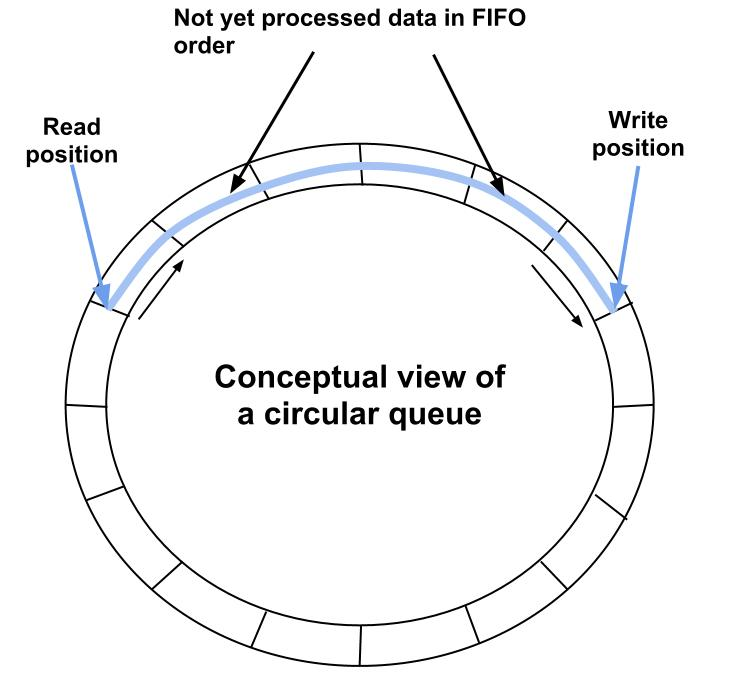
\includegraphics[scale = 0.5]{circularqueue.jpg}
\captionof{figure}{This is the overview of the fixed length queue.}
}
\end{minipage}
\medskip
\end{center}
\section{Measurement}

Because the digital debug is a very time consuming process, real time processing with debug information is not impossible, so I output it the voltage directly and use the fft in the oscilloscope to do the fft analysis.

Below is the result, the feeding signal is the white noise from the laboratory signal generator. And the sampling frequency is 10khz, which means the cutoff frequency is at around 2khz.
\begin{center}
\begin{minipage}[t]{\linewidth}
%\label{fig:main}

{
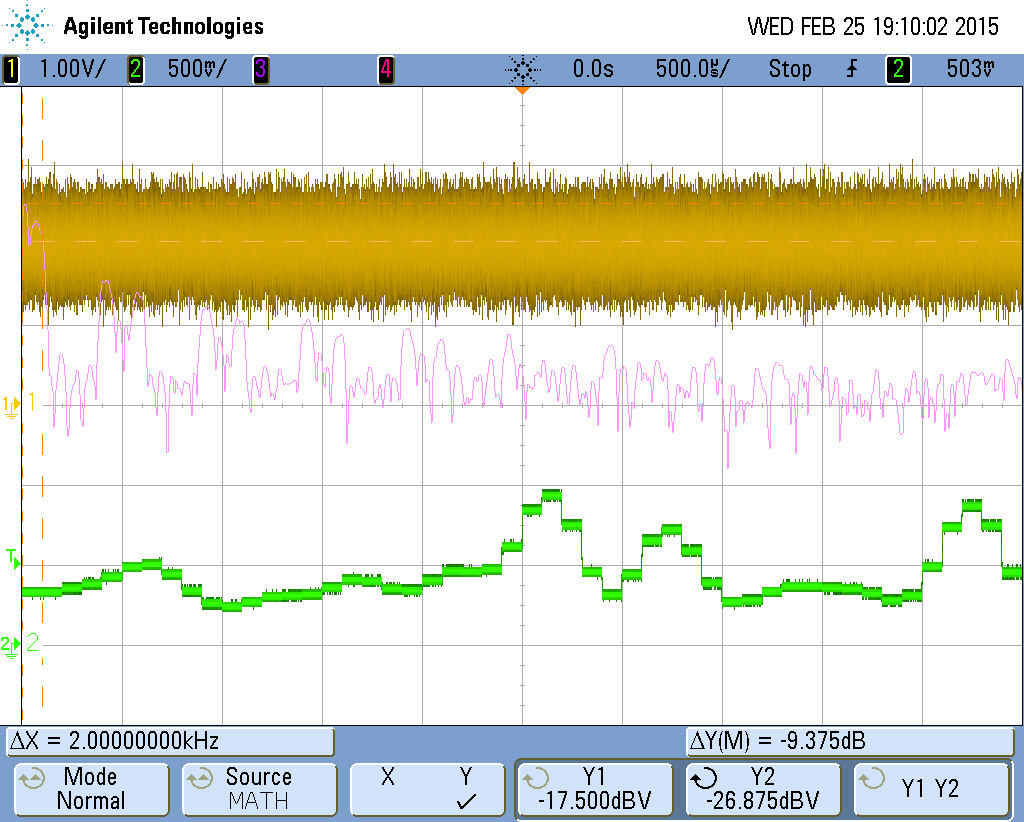
\includegraphics[scale = 0.5]{re13.png}
\captionof{figure}{This is the result. As we can see, at the cutoff frequency the attenuation ratio is 9.3db.}
}
\end{minipage}
\medskip
\end{center}
\subsection{Measurment}

As we can see, at the cutoff frequency the attenuation ratio is 9.3 db instead of 3db. And before the cutoff frequency the filter keeps the output at a relative high and flatten level.
\subsection{Calculation of cutoff frequency}

According to the handout, the cutoff frequency is at 0.2 of the sampling rate, and because the interrupt frequency is at 10khz, we will get cutoff frequency at around 2khz.


\end{document}
